\begin{center}
	\LARGE
	Uden hjælpemidler
\end{center}
\begin{opgavetekst}{Opgave 1}
	Grafen for en eksponentialfunktion $f$ med forskriften
	\begin{align*}
		f(x) = b\cdot a^x
	\end{align*}
	kan ses på Figur \ref{fig:expgraf}
	\begin{figure}[H]
		\centering
		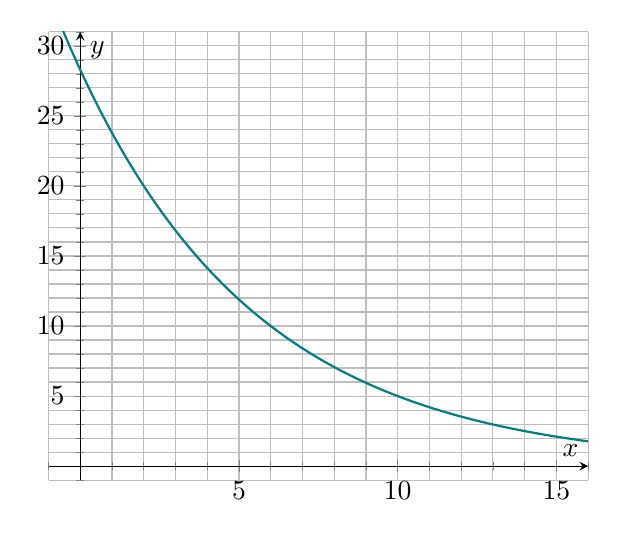
\begin{tikzpicture}
		\begin{axis}[
		axis lines = center, 
		xmin = -1, xmax = 16,
		ymin = -1, ymax = 31,
		xlabel = $x$, ylabel = $y$, 
		xtick = {-5,0,...,15,20},
		ytick = {-5,0,...,30,35},
		grid = both, 
		minor tick num = 4,
		]
			\addplot[color = teal, thick, domain = -1:31, samples = 400] {28.284*0.84090^x};
		\end{axis}
		\end{tikzpicture}
		\caption{Graf for funktionen $f$.}
		\label{fig:expgraf}
	\end{figure}
	\phantom{h}
\end{opgavetekst}
\begin{delopgave}{1}
	Bestem halveringskonstanten for $f$.  
\end{delopgave}
%
%
%
%
%
%
\begin{opgavetekst}{Opgave 2}
	En funktion $g$ har forskriften
	\begin{align*}
		g(x) = b\cdot a^x.
	\end{align*}
	Det oplyses desuden, at $g$ skærer gennem punkterne $(2,10)$ og $(5,80)$. 
\end{opgavetekst}
\begin{delopgave}{1}
	Bestem tallene $a$ og $b$. 
\end{delopgave}
\begin{delopgave}{2}
	Bestem vækstraten for $g$ og forklar, hvad dette tal betyder for væksten af $g$. 
\end{delopgave}
%
%
%
%
%
\begin{opgavetekst}{Opgave 3}
	Tre funktioner $f$, $g$ og $h$ er givet ved henholdsvis
	\begin{align*}
		f(x) &= 2x^2, \\
		g(x) &= 1.5x^{0.5}, \\
		h(x) &= 2x^{-0.3}.
	\end{align*}
	Graferne $A$, $B$ og $C$ tilsvarer hver en af disse funktioner. Disse kan ses på Figur \ref{fig:potens}
	\begin{figure}[H]
		\centering
		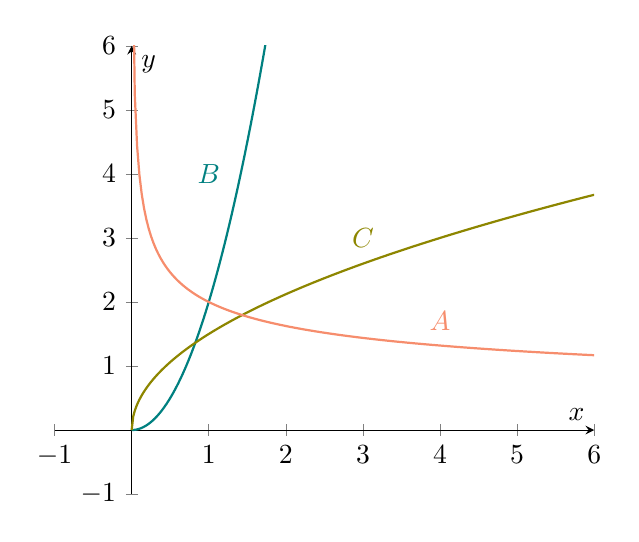
\begin{tikzpicture}
		\begin{axis}[
		axis lines = center, 
		xmin = -1, xmax = 6,
		ymin = -1, ymax = 6,
		xlabel = $x$, ylabel = $y$, 
		xtick = {-1,0,...,6,7},
		ytick = {-1,0,...,6,7},
		]
			\addplot[color = teal, thick, domain = 0.0:6, samples = 200] {2*x^2};
			\addplot[color = olive, thick, domain = 0.0:6, samples = 300] {1.5*x^0.5};
			\addplot[color = Melon, thick, domain = 0.01:6, samples = 200] {2*x^(-0.3)};
			\node[color = Melon] at (axis cs: 4,1.7) {$A$};
			\node[color = teal] at (axis cs: 1,4) {$B$};
			\node[color = olive] at (axis cs: 3,3) {$C$};
		\end{axis}
		\end{tikzpicture}
		\caption{De tre grafer $A$, $B$ og $C$ for funktionerne $f$, $g$ og $h$.}
		\label{fig:potens}
	\end{figure}
	\phantom{h}
\end{opgavetekst}
\begin{delopgave}{1}
	Afgør, hvilke af graferne $A$, $B$ og $C$, der passer til funktionerne $f$, $g$ og $h$. Begrund dit svar. 
\end{delopgave}
\begin{delopgave}{2}
	Bestem $x$-koordinaten i punktet $P(x,8)$, der ligger på grafen $B$. 
\end{delopgave}
%
%
%
%
%
\begin{opgavetekst}{Opgave 4}
	Funktionen $f:\mathbb{R}_{\geq 0} \to \mathbb{R}_{\geq 0}$ givet ved
	\begin{align*}
		f(x) = \ln(\sqrt{2x+1})
	\end{align*}
	er bijektiv. 
\end{opgavetekst}
\begin{delopgave}{1}
	Bestem forskriften for funktionen $f^{-1}$.
\end{delopgave}
%
%
%
%
%
\begin{opgavetekst}{Opgave 5}
	Grafen for en funktion $g:]-5,5] \to ]-5,4[$ kan ses på Figur \ref{fig:surinj}.
	\begin{figure}[H]
		\centering
		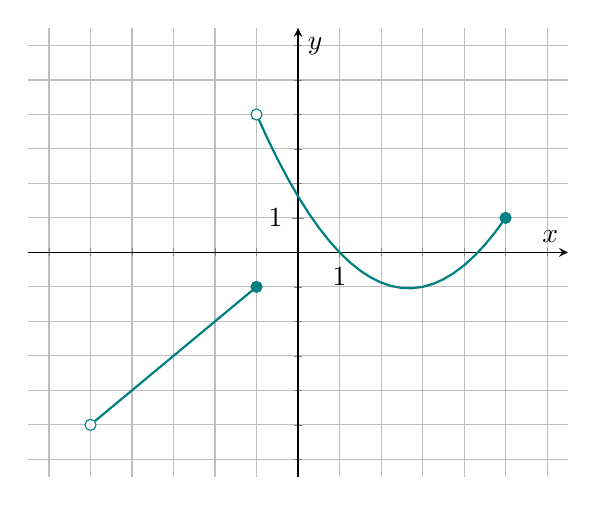
\begin{tikzpicture}
		\begin{axis}[
		axis lines = center, 
		xmin = -6.5, xmax = 6.5,
		ymin = -6.5, ymax = 6.5,
		xlabel = $x$, ylabel = $y$, 
		xtick = {-17,-8,...,1,10},
		ytick = {-17,-8,...,1,10},
		grid = both, 
		minor tick num = 8,
		]
			\addplot[color = teal, thick, domain = -5:-1] {x};
			\filldraw[color = white] (axis cs: -5,-5) circle (2pt);
			\draw[color = teal] (axis cs: -5,-5) circle (2pt);
			\filldraw[color = teal] (axis cs: -1,-1) circle (2pt);
			\addplot[color = teal, thick, domain = -1:5] {0.375*x^2-2*x+1.625};
			\filldraw[color = white] (axis cs: -1,4) circle (2pt);
			\draw[color = teal] (axis cs: -1,4) circle (2pt);
			\filldraw[color = teal] (axis cs: 5, 1) circle (2pt);
		\end{axis}
		\end{tikzpicture}
		\caption{Graf for funktionen $g$.}
		\label{fig:surinj}
	\end{figure}
	\phantom{h}
\end{opgavetekst}
\begin{delopgave}{1}
	Afgør, om $g$ er surjektiv, injektiv eller bijektiv. 
\end{delopgave}
\begin{delopgave}{2}
	Bestem $g(-1)$.
\end{delopgave}
%
%
%
%
%
\newpage
\begin{opgavetekst}{Opgave 6}
	På Figur \ref{fig:trekant} er en trekant $\triangle ABC$ givet. 
	\begin{figure}[H]
		\centering
		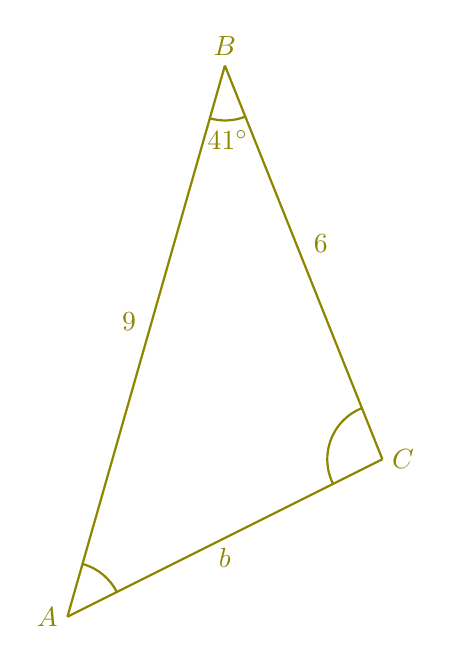
\begin{tikzpicture}
		%A
		\pgfmathsetmacro{\ax}{0}
		\pgfmathsetmacro{\ay}{0}
		%B
		\pgfmathsetmacro{\bx}{2}
		\pgfmathsetmacro{\by}{7}
		%C
		\pgfmathsetmacro{\cx}{4}
		\pgfmathsetmacro{\cy}{2}
		%arc radius
		\pgfmathsetmacro{\arclen}{0.7}
		%c
		\draw[color = olive, thick] (\ax,\ay) -- (\bx,\by) node[midway, anchor = south east] {$9$};
		%b
		\draw[color = olive, thick] (\ax,\ay) -- (\cx,\cy) node[midway, anchor = north] {$b$};
		%a
		\draw[color = olive, thick] (\bx,\by) -- (\cx,\cy) node[midway, anchor = south west] {$6$};
	%	Vinkel A		
		\draw[color = olive, thick] (0.63,0.31) arc (26.57:47.49+26.57:\arclen) 
		node[midway, anchor = south west] {};
	%	Vinkel B
		\draw[color = olive, thick] (1.81,6.33) arc (180 + 74.05:180+74.05+37.75:\arclen)
		 node[midway, anchor = north] {$41^{\circ}$};
	%	Vinkel C
		\draw[color = olive, thick] (3.74,2.65) arc (111.8:111.8+94.76:\arclen)
		 node[midway, anchor = east] {};
		 %Nodes
		 \node[color = olive, anchor = east] at (\ax,\ay) {$A$};
		 \node[color = olive, anchor = south] at (\bx,\by) {$B$};
		 \node[color = olive, anchor = west] at (\cx,\cy) {$C$};
		\end{tikzpicture}
		\caption{Trekant $\triangle ABC$.}
		\label{fig:trekant}
	\end{figure}
	\phantom{h}	 
\end{opgavetekst}
\begin{delopgave}{1}
	Bestem sidelængden $b$, hvor du anvender Tabel \ref{tab:cossintan}. Afrund til to decimaler.
\end{delopgave}
%
%
%
%
%
\begin{opgavetekst}{Opgave 7}
	Et polynomium $p$ er givet ved
	\begin{align*}
		p(x) = (x-5)(x^2-8x+15)
	\end{align*}
\end{opgavetekst}
\begin{delopgave}{1}
	Bestem rødderne for $p$. 
\end{delopgave}
%
%
%%%%%%%%%%%%%%%
%
%
\newpage
\begin{center}
	\LARGE
	Med hjælpemidler
\end{center}

\begin{opgavetekst}{Opgave 8}
	En stykvist defineret funktion $f$ er givet ved
	\begin{align*}
		f(x) := 
		\begin{cases}
			2x+5, \ &\textnormal{ hvis }x < -4, \\
			x^2 - 19, \ &\textnormal{ hvis }-4 \leq x \leq 4,\\
			-2x + 5, \ &\textnormal{ hvis } 4 < x.
		\end{cases}
	\end{align*}
\end{opgavetekst}
\begin{delopgave}{1}
	Tegn grafen for $f$ på intervallet $[-5,5]$.
\end{delopgave}
\begin{delopgave}{2}
	Løs ligningen $f(x) = -8$
\end{delopgave}
%
%
%
%
%
\begin{opgavetekst}{Opgave 9}
	\begin{center}
		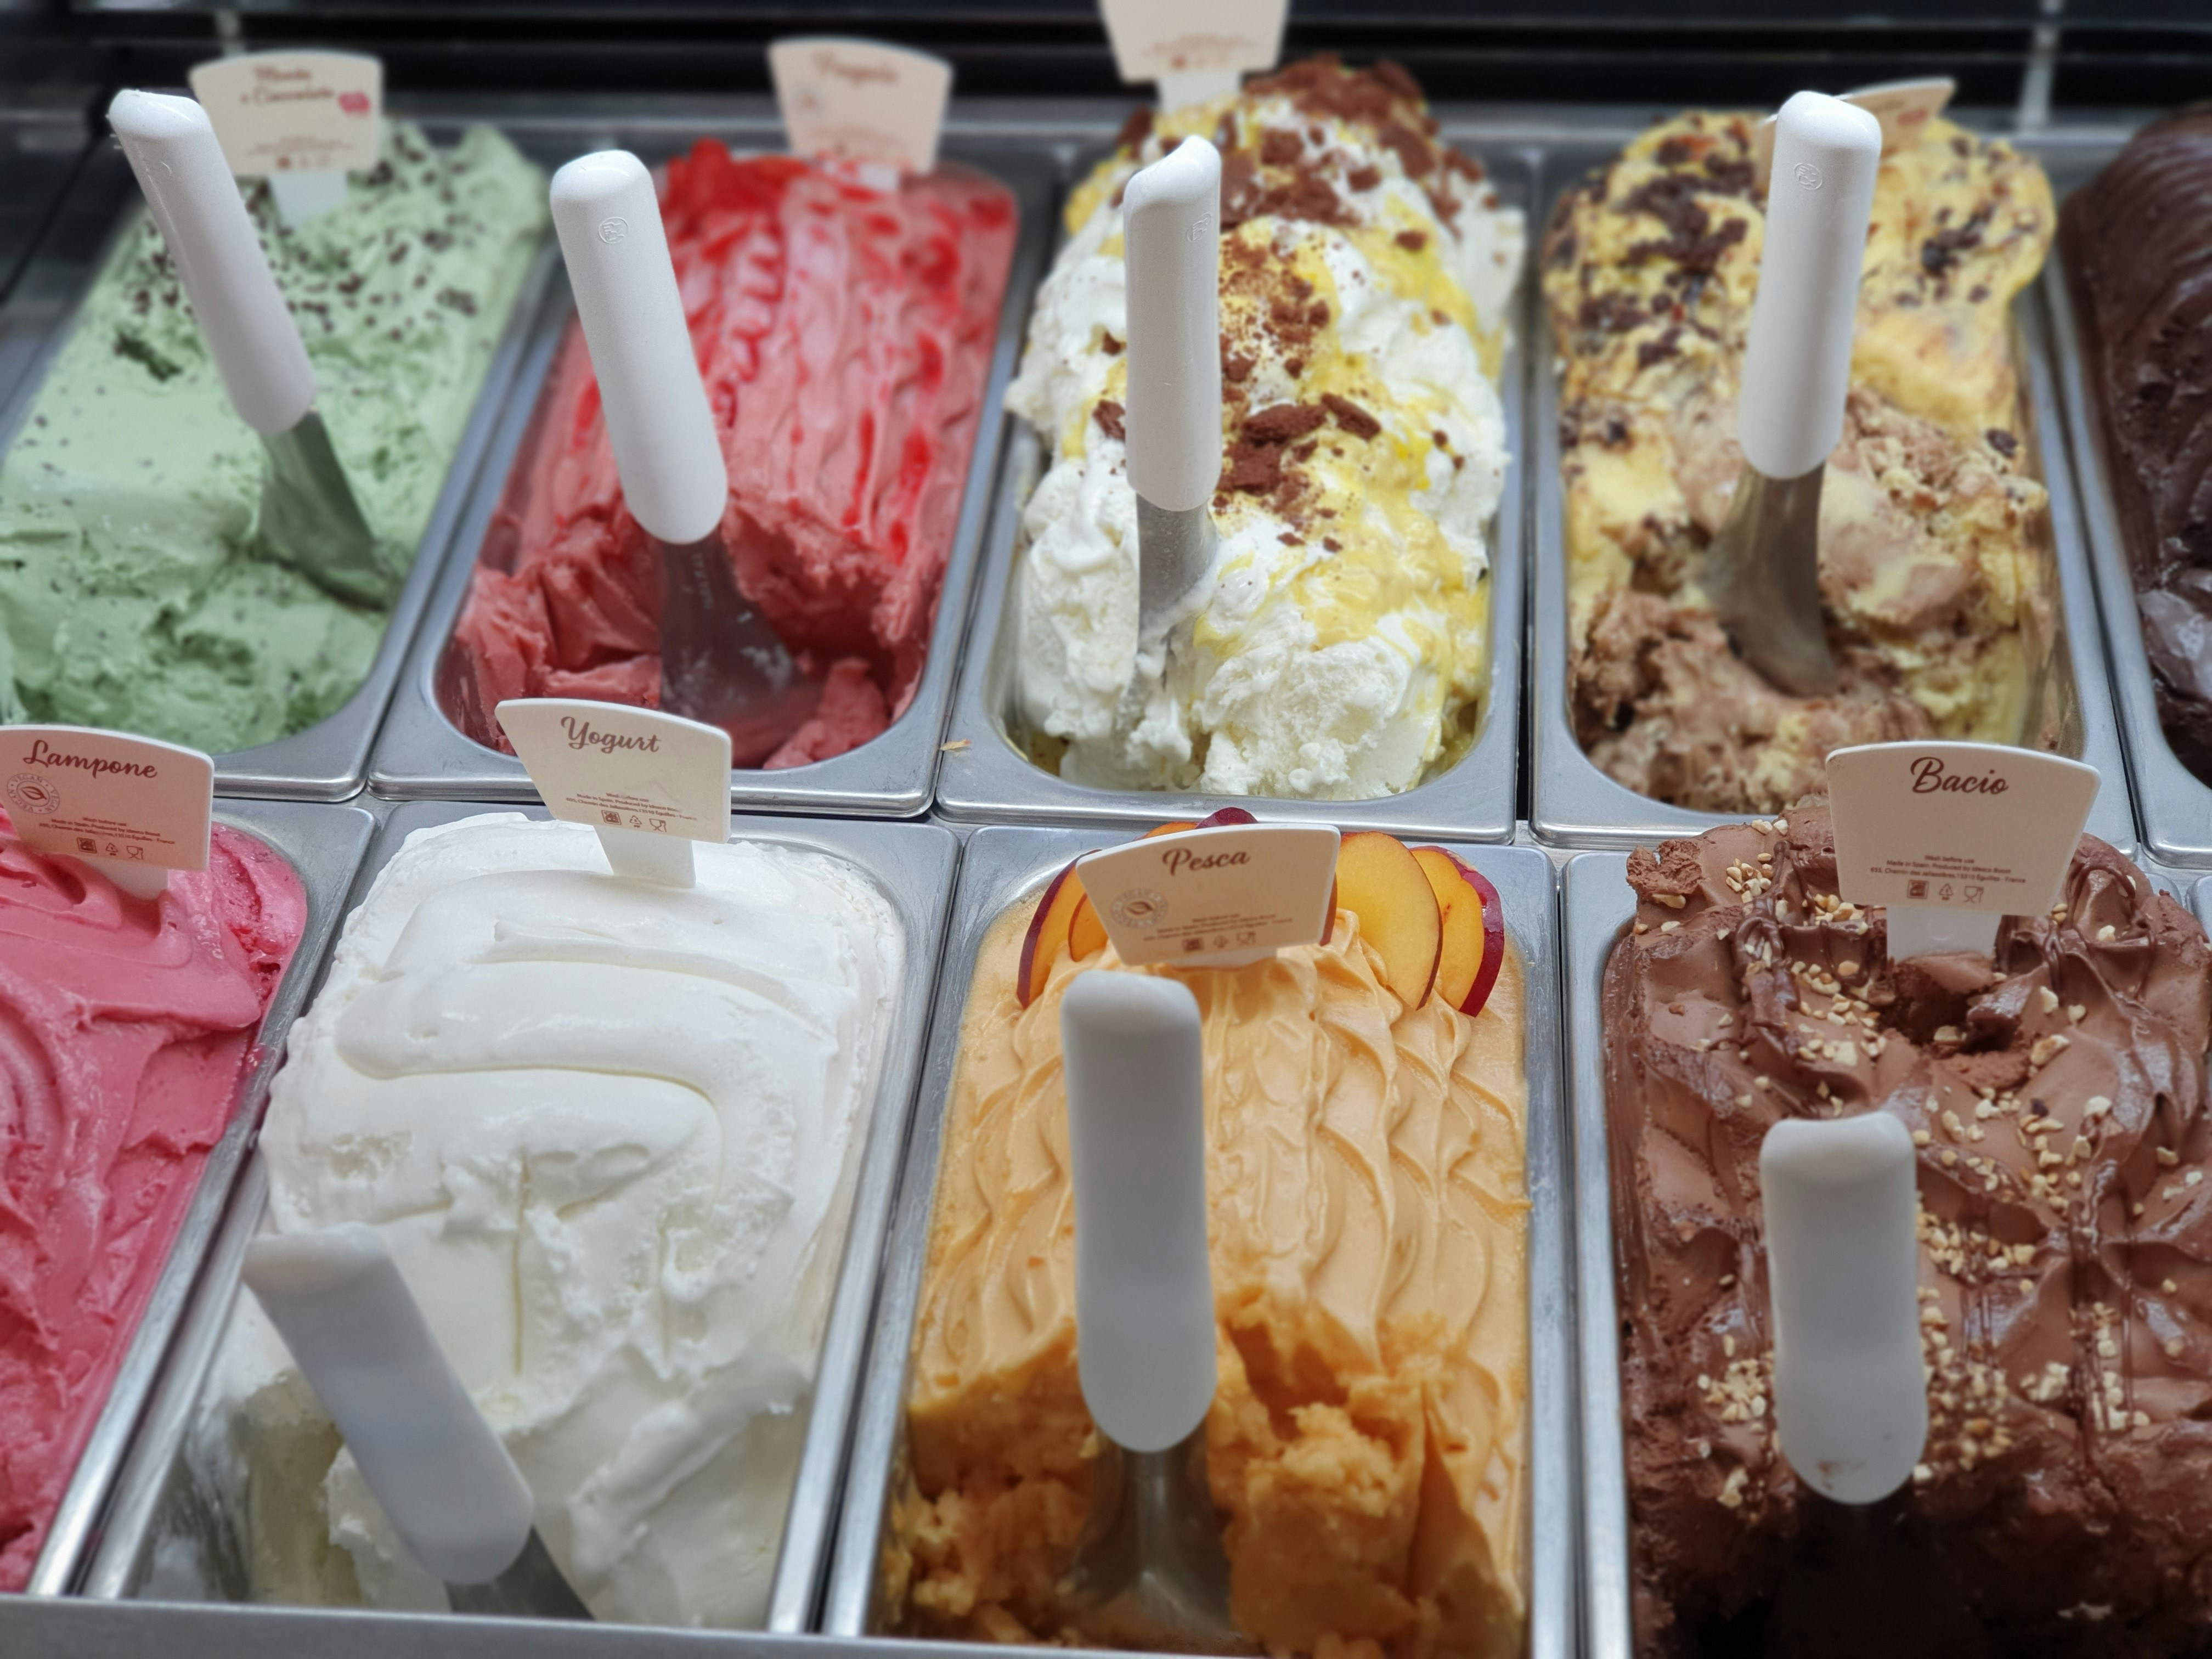
\includegraphics[width = 0.6\textwidth]{Billeder/is}
	\end{center}
	En isproducent har henover en årrække øget deres salg af is. Omsætningen på is kan findes i \href{https://github.com/ChristianJLex/TeachingNotes/raw/master/2025-2026/Data og lign/isnamnam.xlsx}{\color{blue!60} dette datasæt.}
	Det antages, at omsætningen på is kan beskrives ved en sammenhæng af typen
	\begin{align*}
		h(t) = b\cdot a^t,
	\end{align*}
	hvor $h$ er den årlige omsætning i mio. kr. og $t$ er antal år forløbet siden år 2000.
\end{opgavetekst}
\begin{delopgave}{1}
	Anvend regression for at bestemme tallene $a$ og $b$
\end{delopgave}
\begin{delopgave}{2}
	Forklar, hvad tallene $a$ og $b$ betyder for omsætningen på is. 
\end{delopgave}
%
%
%
%
%
\begin{opgavetekst}{Opgave 10}
	Tre ligninger er givet ved
	\begin{align*}
		&2x + 5y + 3z = 1,\\
		&4x + 10y - 4z = 3,\\
		&6x - y + 15z = -4.
	\end{align*}
\end{opgavetekst}
\begin{delopgave}{1}
	Bestem løsningen til ligningssystemet. 
\end{delopgave}
%
%
%
%
%
\newpage
\begin{opgavetekst}{Opgave 11}
	\begin{center}
		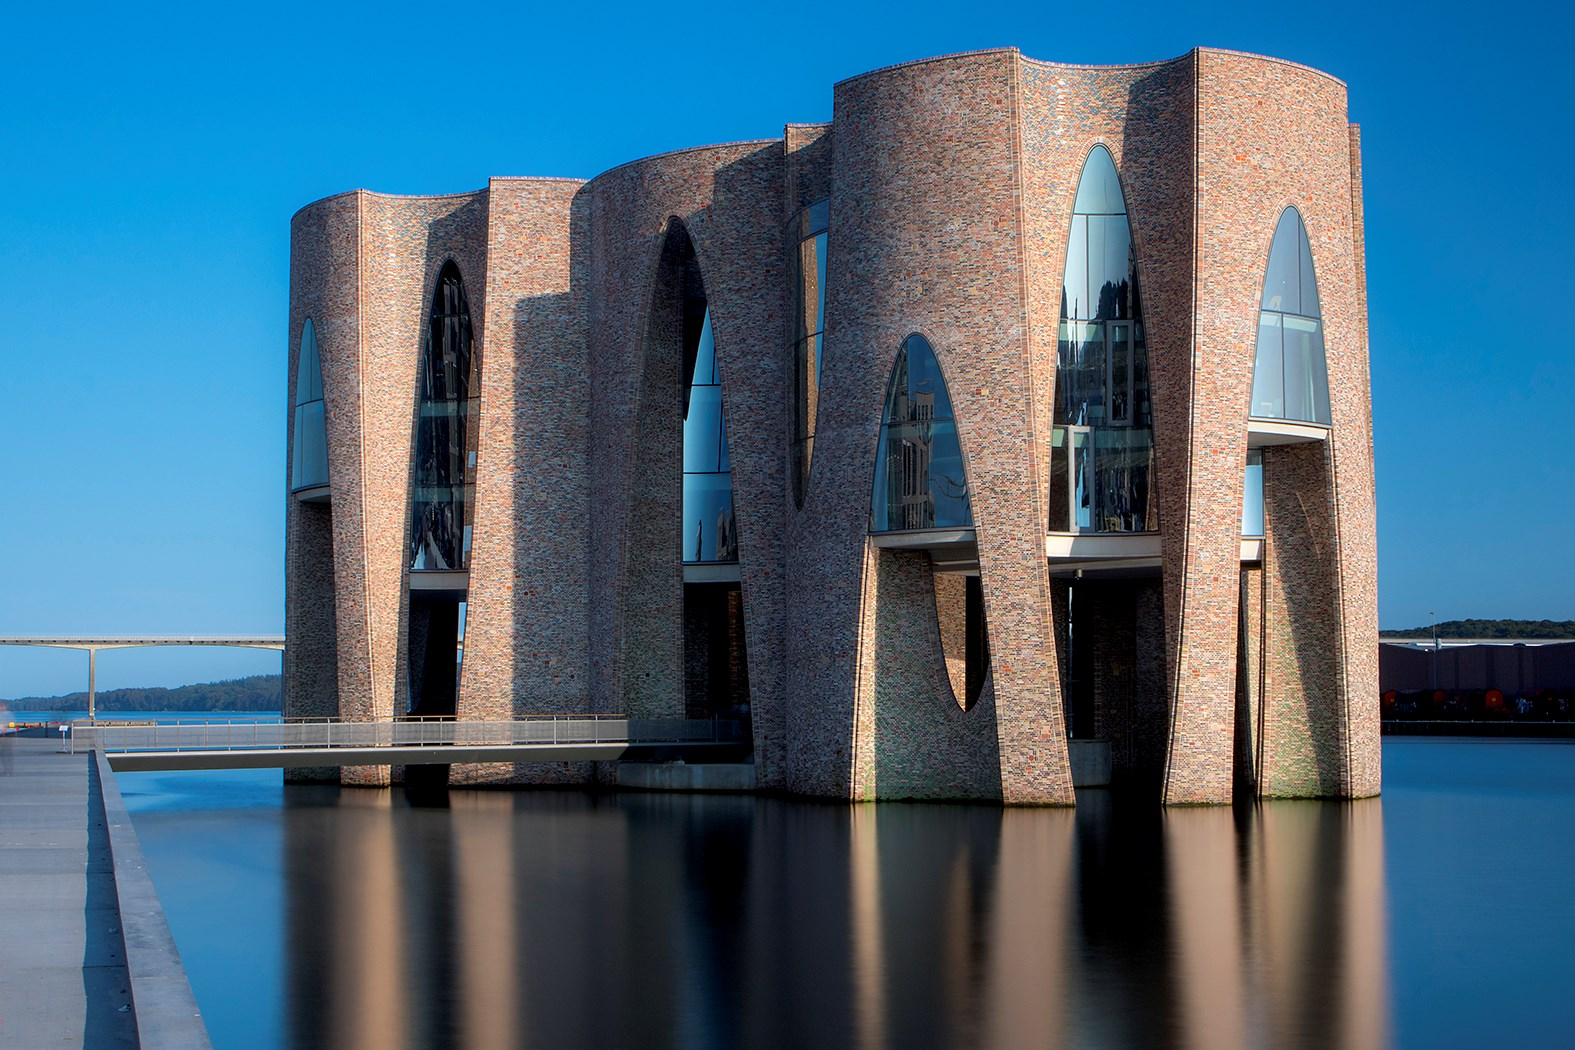
\includegraphics[width = 0.6\textwidth]{Billeder/Fjordenhus}
	\end{center}
	I Vejle ligger Fjordenhus, der som en del af facaden har parabellignende buer. Én af buerne kan ses indlejret i et koordinatsystem på Figur \ref{fig:fjordenhus}.
	\begin{figure}[H]
		\centering
		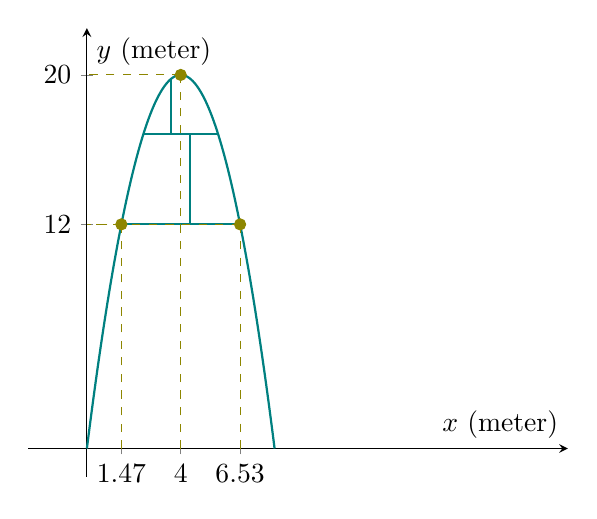
\begin{tikzpicture}
			\begin{axis}[
				axis lines = middle, 
				xmin = -2.5, 
				xmax = 20.5,
				ymin = -1.5,
				ymax = 22.5,
				xlabel = {$x$ (meter)},
				ylabel = {$y$ (meter)},
				xtick = {1.47,4,6.53},
				ytick = {12,20}
			]
				\addplot[color = teal, thick, samples = 150, domain = 0:8] {-1.25*x^2+10*x};
				\draw[color = teal, thick] (axis cs: 1.47,12) -- (axis cs: 6.53,12);
				\draw[color = teal, thick] (axis cs: 2.41,16.84) -- (axis cs: 5.59,16.84);
				\draw[color = teal, thick] (axis cs: 3.6,19.8) -- (axis cs: 3.6,16.84);
				\draw[color = teal, thick] (axis cs: 4.4,16.84) -- (axis cs: 4.4,12);
				\filldraw[color = olive] (axis cs: 1.47,12) circle (2pt);
				\filldraw[color = olive] (axis cs: 6.53,12) circle (2pt);
				\filldraw[color = olive] (axis cs: 4,20) circle (2pt);
				\draw[color = olive, dashed] (axis cs: 1.47,0) -- (axis cs: 1.47,12);
				\draw[color = olive, dashed] (axis cs: 1.47,12) -- (axis cs: 0,12);
				\draw[color = olive, dashed] (axis cs: 6.53,12) -- (axis cs: 0,12);
				\draw[color = olive, dashed] (axis cs: 6.53,12) -- (axis cs: 6.53,0);
				\draw[color = olive, dashed] (axis cs: 4,0) -- (axis cs: 4,20);
				\draw[color = olive, dashed] (axis cs: 4,20) -- (axis cs: 0,20);
			\end{axis}
		\end{tikzpicture}
		\caption{Skitse af facadeparabel på Fjordenhus.}
		\label{fig:fjordenhus}
	\end{figure}
	\phantom{h}
\end{opgavetekst}
\begin{delopgave}{1}
	Bestem en forskrift for den parabel, der fremgår af Figur \ref{fig:fjordenhus}.
\end{delopgave}
\begin{delopgave}{2}
	Afgør, hvor bred facadebuen på Fjordenhus er i vandoverfladen. 
\end{delopgave}
%
%
%
%
%

\phantom{h}
\newpage
\begin{center}
	\LARGE Bilag:
\end{center}
\begin{table}[H]
	\centering
	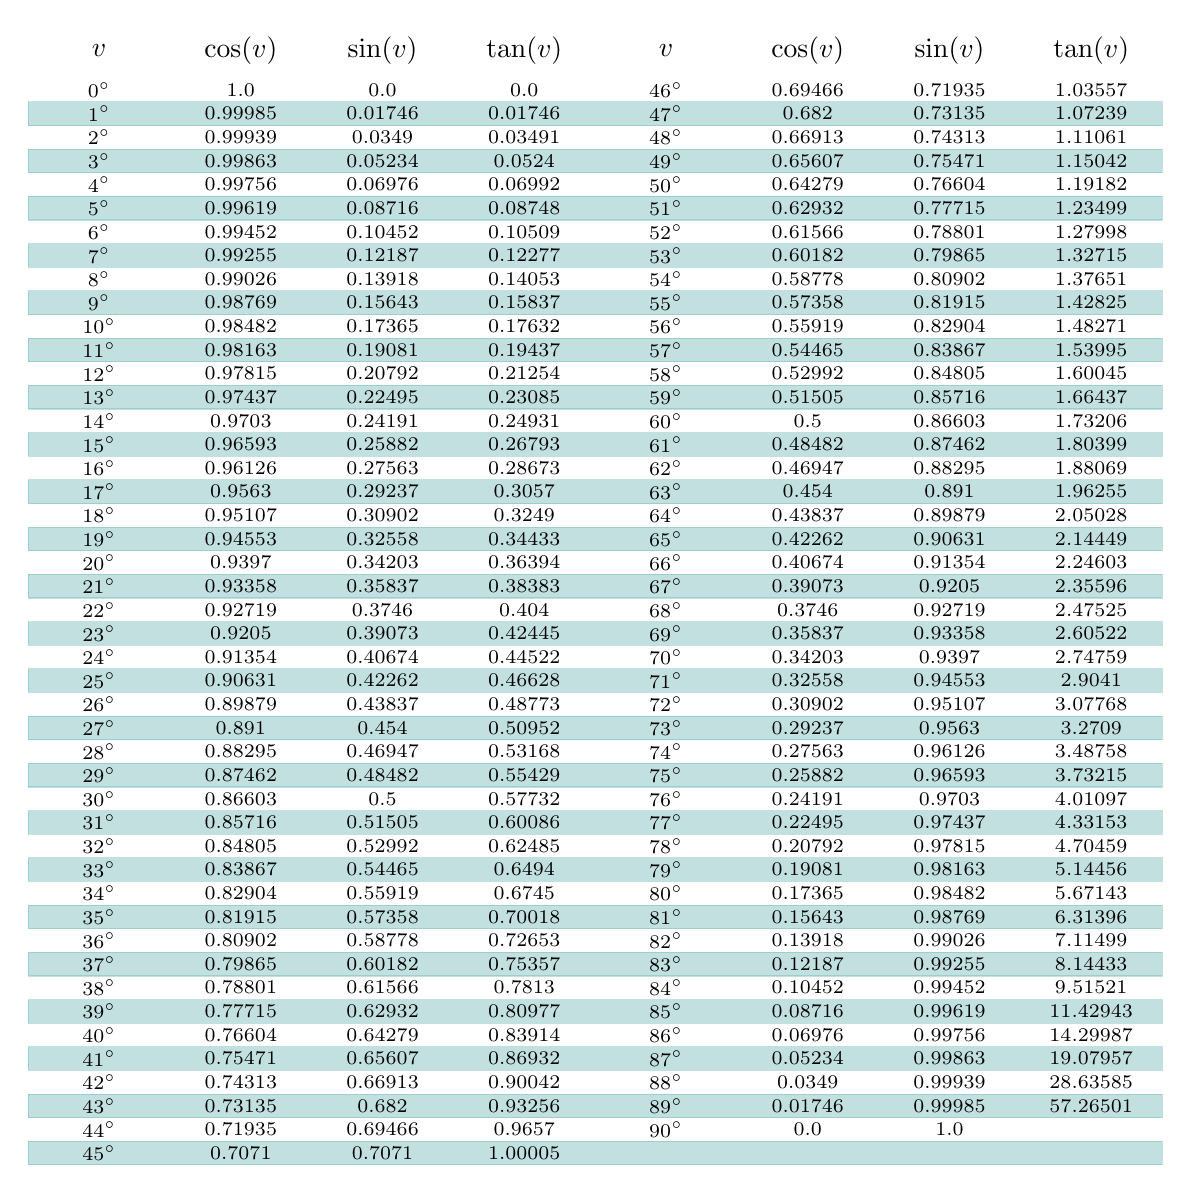
\begin{tikzpicture}
	\node at (0,0) {$v$};
	\node at (2*0.9,0) {$\cos(v)$};
	\node at (4*0.9,0) {$\sin(v)$};
	\node at (6*0.9,0) {$\tan(v)$};
	\node at (8*0.9,0) {$v$};
	\node at (10*0.9,0) {$\cos(v)$};
	\node at (12*0.9,0) {$\sin(v)$};
	\node at (14*0.9,0) {$\tan(v)$};
	\scriptsize
	%Colors
	\foreach \i in {0,...,22}{
		\filldraw[color = teal!60, opacity = 0.4] (-0.9,-0.5-0.3+0.15-\i*0.3*2) rectangle
		 (14*0.9 + 0.9,-0.5-0.3-0.15-\i*0.3*2);
	}
	\foreach \i in {0,...,45}{
		%Macros for evaluating
		\pgfmathsetmacro{\cval}{cos(\i)}
		\pgfmathsetmacro{\sval}{sin(\i)}
		\pgfmathsetmacro{\tval}{tan(\i)}
		%First columns of values
		\node at (0,-0.5-\i*0.3) {$\i^{\circ}$};
		\node at (2*0.9,-0.5-\i*0.3) { \cval };
		\node at (4*0.9,-0.5-\i*0.3) { \sval };
		\node at (6*0.9,-0.5-\i*0.3) { \tval };
	}
	\foreach \i in {46,...,89}{
		%Macros
		\pgfmathsetmacro{\cval}{cos(\i)}
		\pgfmathsetmacro{\sval}{sin(\i)}
		\pgfmathsetmacro{\tval}{tan(\i)}
		%Second column
		\node at (8*0.9,-0.5-\i*0.3 + 46*0.3) {$\i^{\circ}$};
		\node at (10*0.9,-0.5-\i*0.3 + 46*0.3) { \cval };
		\node at (12*0.9,-0.5-\i*0.3 + 46*0.3) { \sval };
		\node at (14*0.9,-0.5-\i*0.3 + 46*0.3) { \tval };
	}
		\pgfmathsetmacro{\cval}{cos(90)}
		\pgfmathsetmacro{\sval}{sin(90)}
		\node at (8*0.9,-0.5-90*0.3 + 46*0.3) {$90^{\circ}$};
		\node at (10*0.9,-0.5-90*0.3 + 46*0.3) { \cval };
		\node at (12*0.9,-0.5-90*0.3 + 46*0.3) { \sval };
	\end{tikzpicture}
	\caption{Tabel over udvalgte værdier for $\cos$, $\sin$ og $\tan$.}
	\label{tab:cossintan}
\end{table}